\documentclass{article}

\usepackage{graphicx}
\usepackage{tikz}
\usepackage{tikzsymbols}
\usetikzlibrary{calc,patterns,shapes.geometric}
\pagestyle{empty}
\usepackage[margin=0pt]{geometry}
\geometry{papersize={14in,12in}}

\def\centerarc[#1](#2)(#3:#4:#5){\draw[#1] ($(#2)+({#5*cos(#3)},{#5*sin(#3)})$) arc (#3:#4:#5);}

\begin{document}
	\begin{figure}
		\centering
		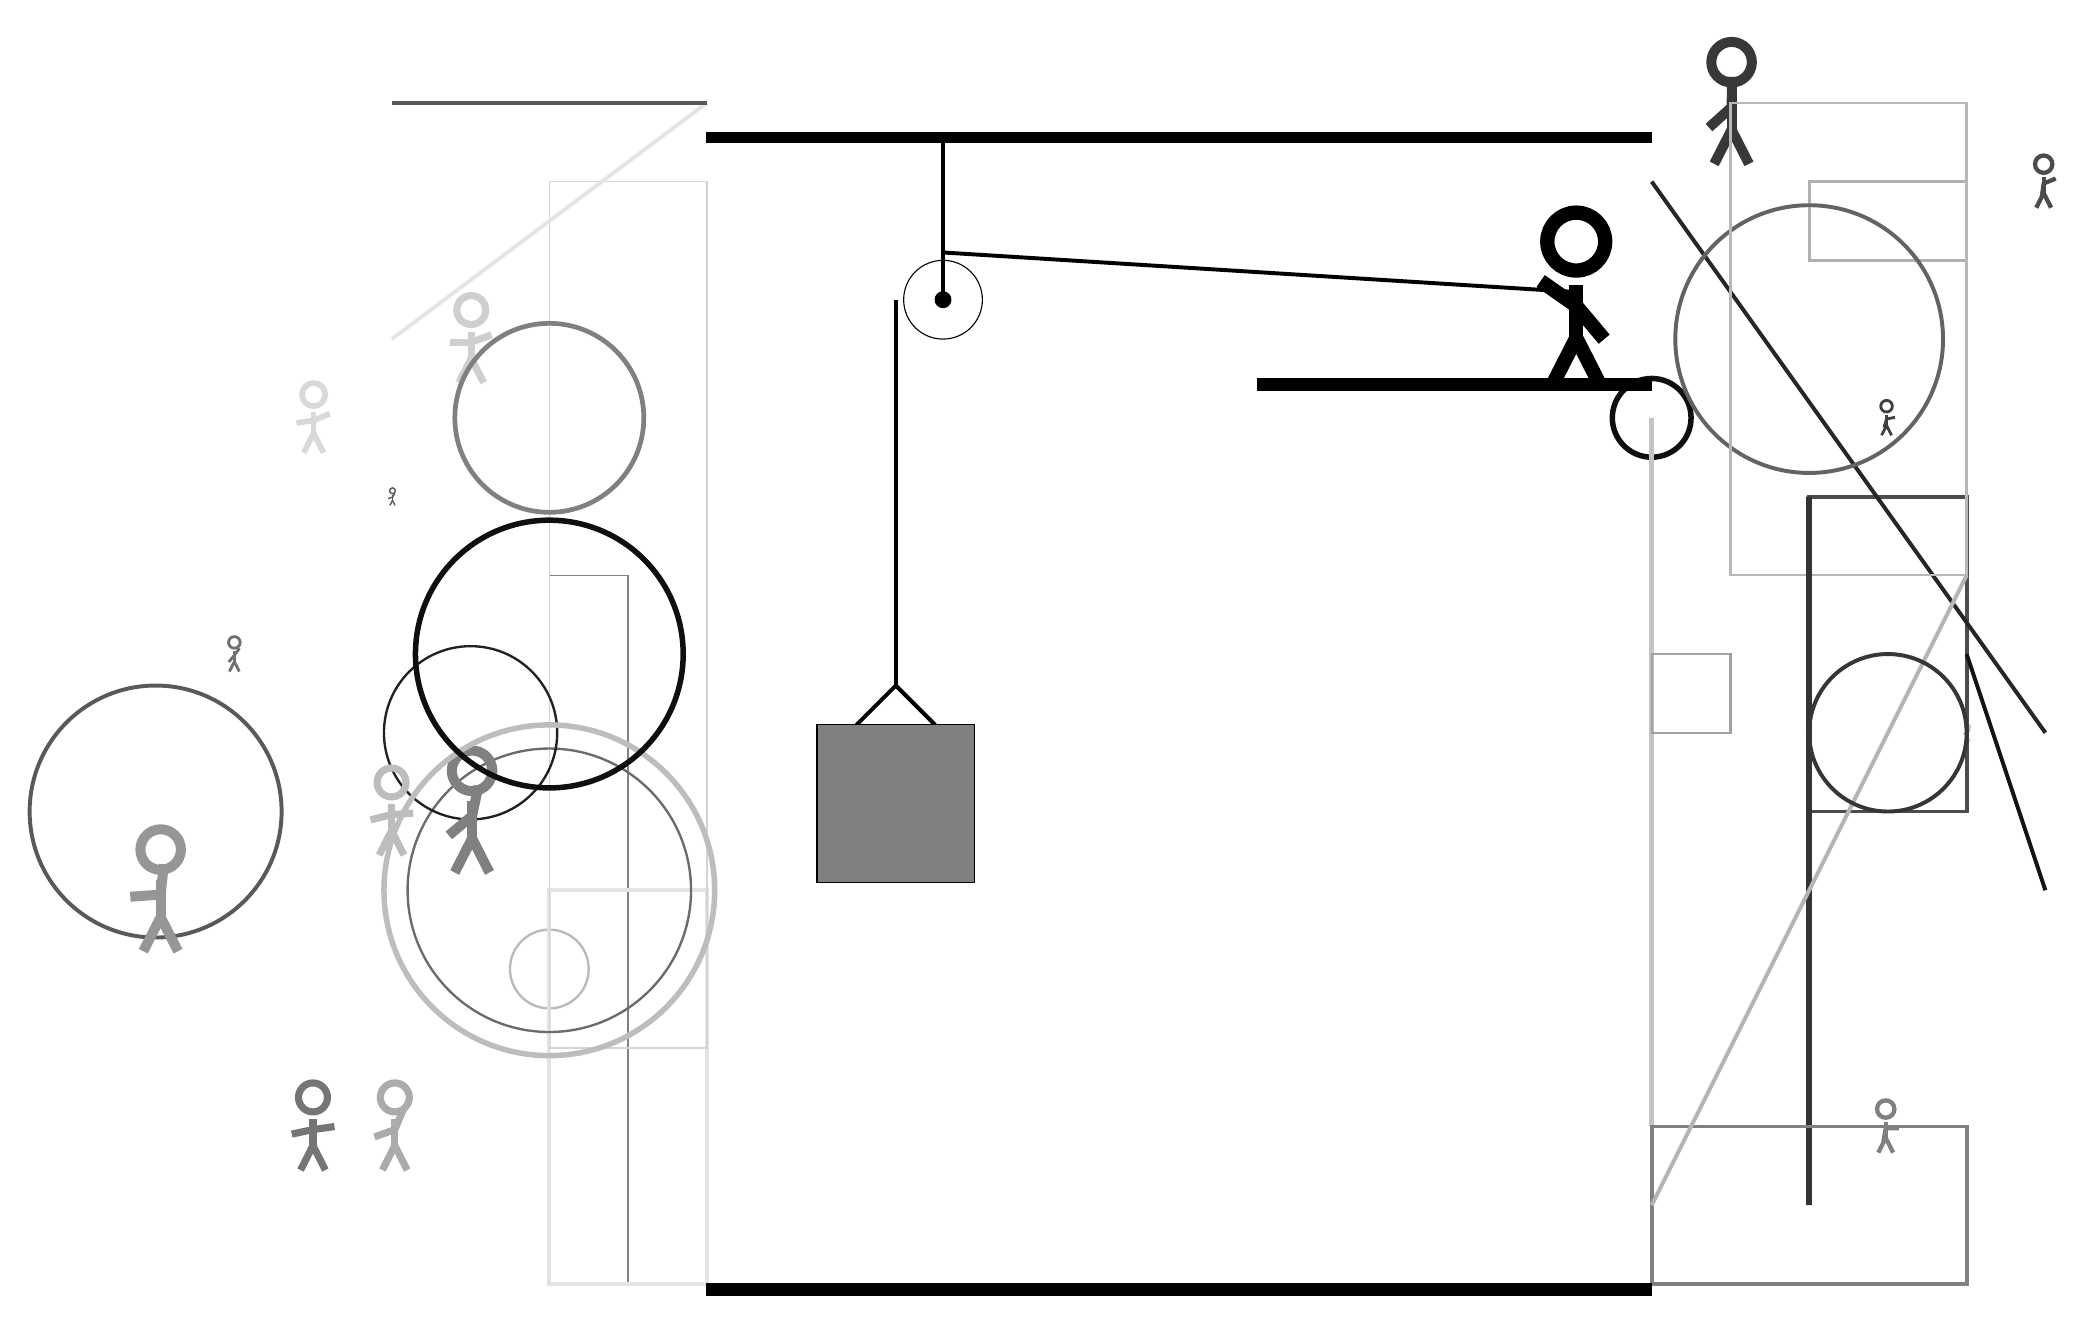
\begin{tikzpicture}
			%%%%% START %%%%%
			
			\draw[fill=black] (-2, 11.5) rectangle (10, 11.625);
			
			\draw (1, 9.5) circle (0.5);
			\draw[fill=black] (1, 9.5) circle (0.1);
			\draw[line width=0.5mm] (1, 11.5) -- (1, 9.5);
			
			\draw[line width=0.5mm](-0.1, 4.1) --  (0.4, 4.6) -- (0.9, 4.1);
			\draw[fill=black!50] (-0.6, 4.1) rectangle (1.4, 2.1);
			
			\draw[line width=0.5mm](0.4, 9.5) -- (0.4, 4.6);
			\centerarc[line width=0.5mm](1, 9.5)(90:180:0.6)
			\draw[line width=0.5mm](1, 10.1) -- (9, 9.6);
			
			\draw[line width=0.2mm, color=black!49] (-3, 6) rectangle (-4, -3);
			
			\node[line width=0.3mm, color=black!75] at (13, 8) {\Strichmaxerl[2][73][12]};
			\node[line width=0.3mm, color=black!78] at (11, 12) {\Strichmaxerl[7][42][89]};
			\node[line width=0.7mm, color=black!15] at (-7, 8) {\Strichmaxerl[4][9][22]};
			\node[line width=0.6mm, color=black!70] at (15, 11) {\Strichmaxerl[3][82][22]};
			\node[line width=0.2mm, color=black!26] at (14, 4) {\Strichmaxerl[1][8][49]};
			\draw [line width=0.7mm, color=black!94](10, 8) circle (0.5);
			
			\draw[line width=0.5mm, color=black!70] (12, 7) rectangle (14, 3);
			\draw [line width=0.3mm, color=black!27](-4, 1) circle (0.5);
			\draw[line width=0.5mm, color=black!11] (-4, -3) rectangle (-2, 2);
			\draw[line width=0.2mm, color=black!17] (-4, 11) rectangle (-2, 0);
			
			\node[line width=0.5mm, color=black!66] at (-6, 7) {\Strichmaxerl[1][17][58]};
			\node[line width=0.5mm, color=black!54] at (-7, -1) {\Strichmaxerl[5][12][8]};
			
			\draw[line width=0.5mm, color=black!92](15, 2) -- (14, 5);
			\draw [line width=0.3mm, color=black!58](-4, 2) circle (1.8);
			\draw[line width=0.4mm, color=black!31] (12, 11) rectangle (14, 10);
			
			\draw [line width=0.3mm, color=black!87](-5, 4) circle (1.1);
			\node[line width=0.2mm, color=black!50] at (-5, 3) {\Strichmaxerl[7][40][78]};
			\draw [line width=0.5mm, color=black!65](-9, 3) circle (1.6);
			\draw [line width=0.7mm, color=black!26](-4, 2) circle (2.1);
			\draw[line width=0.7mm, color=black!23] (10, 8) rectangle (10, -1);
			\node[line width=0.5mm, color=black!41] at (-9, 2) {\Strichmaxerl[7][4][84]};
			
			\draw[line width=0.5mm, color=black!85](10, 11) -- (15, 4);
			\draw[line width=0.5mm, color=black!10](-2, 12) -- (-6, 9);
			\node[line width=0.2mm, color=black!50] at (13, -1) {\Strichmaxerl[3][80][1]};
			
			\draw [line width=0.5mm, color=black!61](12, 9) circle (1.7);
			\draw[line width=0.3mm, color=black!28] (11, 12) rectangle (14, 6);
			\node[line width=0.5mm, color=black!19] at (-5, 9) {\Strichmaxerl[5][0][20]};
			\draw[line width=0.7mm, color=black!80] (12, 7) rectangle (12, -2);
			\draw[line width=0.5mm, color=black!50] (10, -1) rectangle (14, -3);
			\node[line width=0.7mm, color=black!56] at (-8, 5) {\Strichmaxerl[2][50][54]};
			\draw[line width=0.3mm, color=black!37] (11, 4) rectangle (10, 5);
			\draw[line width=0.5mm, color=black!29](10, -2) -- (14, 6);
			\node[line width=0.4mm, color=black!33] at (-6, -1) {\Strichmaxerl[5][20][67]};
			\draw [line width=0.5mm, color=black!79](13, 4) circle (1.0);
			\draw [line width=0.6mm, color=black!50](-4, 8) circle (1.2);
			\node[line width=0.3mm, color=black!26] at (-6, 3) {\Strichmaxerl[5][14][4]};
			
			\draw[line width=0.5mm, color=black!65](-2, 12) -- (-6, 12);
			\draw [line width=0.7mm, color=black!94](-4, 5) circle (1.7);
			
			\node at (9, 9.5) {\Strichmaxerl[10][-35][-50]};
			\draw[fill=black] (5, 8.5) rectangle (10, 8.35);
			
			\draw[fill=black] (-2, -3) rectangle (10, -3.15);
			
			%%%%% END %%%%%
		\end{tikzpicture}
	\end{figure}	
\end{document}